% Перестроение расчетной сетки в трехмерном случае.
\newpage
\section*{Глава 2. Перестроение поверхностной расчетной сетки в трехмерном случае} % выключить номер первой главы
\addcontentsline{toc}{section}{Глава 2. Перестроение поверхностной расчетной сетки в трехмерном случае} % но добавить ее в оглавление
\addtocounter{section}{1}                                                                             % а теперь и счетчик продвинуть
\setcounter{subsection}{0}
\setcounter{figure}{0}
\setcounter{equation}{0}
\setcounter{table}{0}
\setcounter{theorem}{0}
\setcounter{lemma}{0}
\setcounter{definition}{0}

В этой главе исследуется перестроение поверхностной расчетной сетки в трехмерном случае применительно к моделированию обледенения \cite{Meshcheryakov2023GeoEvo}.
Рассматриваются известные методы перестроения как аналоги рассмотренным ранее двумерным методам.
Рассматриваются дополнительные аспекты повышения точности и стабильности перестроения, а также различные виды сглаживания, выполняемые на поверхностных расчетных сетках.
Предлагается новый метод перестроения поверхностной расчетной сетки как обобщение двумерного метода окрестностей на трехмерный случай, приводятся формулы для нахождения новых положений узлов расчетной сетки в общем случае.

Задача перестроения поверхностной расчетной сетки в пространстве является центральной задачей при расчете обледенения поверхности.
В дальнейшем перестроение поверхностной сетки будем рассматривать в применении к моделированию процесса обледенения.
Входными данными этой задачи является масса (или объем) накопленного льда в каждой ячейке расчетной сетки.
В ходе решения расчетная сетка должна быть перестроена таким образом, чтобы объем, заметаемый ячейкой в процессе перестроения, соответствовал накомленному в ней льду.

В этой главе ячейки расчетной сетки представлены треугольниками.
Треугольник с вершинами $A$, $B$, $C$, обозначаемый $Tri(A, B, C)$, будем определять как ГМТ\label{abbr:gmt-3} $\overline{P}(\beta, \gamma)$ в пространстве, заданное следующим образом:

\begin{equation}\label{eqn:text_1_geo_prim_triangle}
	\left\{
		\begin{aligned}
			& \overline{P}(\beta, \gamma) = \overline{A} + \beta \overline{AB} + \gamma \overline{AC}, \ \beta \in \mathbb{R}, \ \gamma \in \mathbb{R} \\
			& \beta \ge 0 \\
			& \gamma \ge 0 \\
			& \beta + \gamma \le 1
		\end{aligned}
	\right.
\end{equation}

Рассмотрим архитектуру поверхностной неструктурированной расчетной сетки, используемой для моделирования обледенения.
Элементами расчетной сетки являются узлы $N \in \mathscr{N}$, ребра $E \in \mathscr{E}$ и ячейки $F \in \mathscr{F}$, имеющие форму треугольников.
Для удобства каждый элемент сетки связан через ссылки со всеми своими инцидентными элементами: так связаны между собой инцидентные узлы и ребра, узлы и ячейки, ребра и ячейки (см. рис.~\ref{fig:text_1_remesh3_architecture}).
Множество инцидентных узлов рассматриваемого ребра $E$ или ячейки $F$ будем обозначать $\mathscr{N}(E)$ и $\mathscr{N}(F)$ соответственно, множество инцидентных ребер рассматриваемого узла $N$ или ячейки $F$ будем обозначать $\mathscr{E}(N)$ и $\mathscr{E}(F)$ соответственно, множество инцидентных ячеек рассматриваемого узла $N$ или ребра $E$ будем обозначать $\mathscr{F}(N)$ и $\mathscr{F}(E)$ соответственно.

\begin{figure}[ht]
\centering
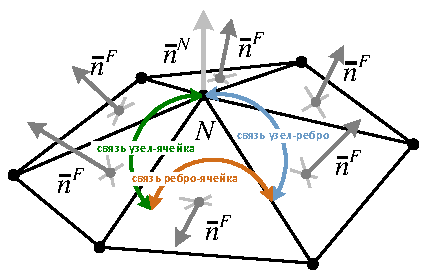
\includegraphics[width=0.5\textwidth]{fig/3dr_architecture.pdf}
\singlespacing
\captionstyle{center}\caption{Архитектура расчетной сетки.}
\label{fig:text_1_remesh3_architecture}
\end{figure}

К расчетной сетке предъявляются следующие требования.
Во-первых, сетка должна быть целостной, то есть каждое ребро имеет ровно два инцидентных узла, отсутствуют изолированные и висячие узлы, а также отсутствуют ребра без инцидентных ячеек.
Во-вторых, все ячейки должны представлять собой треугольники (это гарантирует, что ячейка является плоской, так как четыре и более произвольных узлов могут не лежать в одной плоскости).
Если каждое ребро имеет ровно две инцидентные ячейки, то сетка является замкнутой.

\begin{equation}\label{eqn:text_1_remesh3_arch}
\begin{cases}
\forall N \implies |\mathscr{E}(N)| > 2, |\mathscr{F}(N)| > 2 \\
\forall E \implies |\mathscr{N}(E)| = 2, |\mathscr{F}(E)| = 2 \\
\forall F \implies |\mathscr{N}(F)| = 3, |\mathscr{E}(F)| = 3 \\
\end{cases}
\end{equation}

В качестве дополнения также будем требовать, чтобы сетка представляла собой двустороннюю поверхность, то есть для каждой ячейки $F$ однозначно определена нормаль к поверхности $\overline{n}^F_F$.
Также никакие два узла сетки не совпадают и отсутствуют ячейки с нулевой площадью (так как это сделает невозможным вычислений нормалей).
Для узла сетки $N$ будем рассматривать понятие нормали к поверхности и определять эту нормаль по аналогии с двумерным случаем как
\begin{equation}
\overline{n}_N^N = \frac{\sum_{F \in \mathscr{F}(N)}{\overline{n}_F^F} }{ \left| \sum_{F \in \mathscr{F}(N)}{\overline{n}_F^F} \right| }
\end{equation}

%---------------------------------------------------------------------------------------------------

\subsection{Классические методы перестроения поверхности}

Центральная задача перестроения поверхностной сетки из-за накопления льда внутри ячеек выглядит следующим образом.
Пусть известно, что в результате численного решения задачи ледообразования конечно-объемным методом \cite{Beaugendre2003Ice} в каждой ячейке $F$ сетки была вычислена масса накопленного льда ($m_F$).
Будем считать плотность льда постоянной, то есть в каждой ячейке также известен объем накопленного льда $V_F = \frac{m_F}{\rho_{ice}}$.
Для каждого узла сетки $N$ требуется найти его новое положение в пространстве $N'$, чтобы для каждой ячейки $F = ABC$ объем пространства, ограниченный фигурой $ABCA'B'C'$, соответствовал объему льда, накопленному в этой ячейке.
Таким образом, поставновка задачи в трехмерном случае аналогично двумерной постановке.
В этом случае будем говорить о перестроении расчетной сетки по объему накопленного льда $V_F$ ($\forall F \in \mathscr{F}$).

Следует отметить, что поставленная задача может не иметь точного решения, и в этом случае следует стремиться к минимизации ошибки по объему (когда фактически образовавшийся объем льда в ячейке $F = ABC$ не сильно отличается от целевого объема, то есть разница $\Delta_F = V_{ABCA'B'C'} - V_F$ мала).

Задачу определения новых положений узлов расчетной сетки можно разделить на две задачи: определение направлений смещения узлов и определение величин смещения.
Простейшие классические методы перестроения выполняются в предположении, что направление смещения узла $N$ совпадает с нормалью, проведенной из этого узла $\overline{n}_N^N$.
Таким образом, необходимо лишь определить величину смещения.

\begin{figure}[h]
\centering
\begin{tabular}{ll}
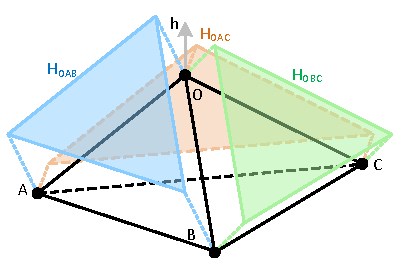
\includegraphics[width=0.43\textwidth]{fig/3dr_prisms.pdf}
&
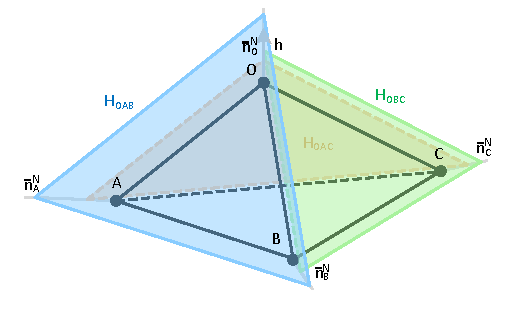
\includegraphics[width=0.52\textwidth]{fig/3dr_pyramids.pdf}
\end{tabular}
\singlespacing
\captionstyle{center}\caption{Перестроение поверхности с помощью метода призм (слева) и пирамид (справа).}
\label{fig:text_1_remesh3_rect}
\end{figure}

\subsubsection{Метод призм}

В качестве первого метода перестроения поверхностной расчетной сетки в трехмерном пространстве рассмотрим метод призм, иллюстрация которого приведена на рис.~\ref{fig:text_1_remesh3_rect} слева (в двумерной постановке аналогом этого метода является метод прямоугольников).
В этом методе входными данными является объем накопленного льда в каждой ячейке сетки ($V_F$).
На первым шаге в каждой ячейке ищется толщина ледяного покрова в предположении, что лед в пределах одной ячейки имеет форму призмы, и ячейка является основанием этой призмы.
Тогда толщина ледяного покрова равняется $H_F = \frac{V_F}{S_F}$, где $S_F$ -- площадь ячейки.
После чего величина смещения каждого узла вычисляется как среднее арифметическое высот ледяного покрова во всех инцидентных ячейках:
\begin{equation}
h_N = \frac{1}{|\mathscr{F}(N)|} \sum_{F \in \mathscr{F}(N)}{H_F}.
\end{equation}

\subsubsection{Заметаемый объем при параллельном смещении ячейки}

Для рассмотрения второго метода перестроения расчетной сетки приведем решение следующей задаче.

Рассмотрим треугольник $Tri(A, B, C)$.
Пусть также известно направление единичной нормали этого треугольника $\overline{n}$, а также направления движения трех его вершин $\overline{n}_A$, $\overline{n}_B$, $\overline{n}_C$.
Пусть на расстоянии $h$ от плоскости $ABC$ проходит параллельная плоскость, пересекающая направления $\overline{n}_A$, $\overline{n}_B$, $\overline{n}_C$ в точках $A'$, $B'$, $C'$ соответственно.
Требуется найти зависимость объема полученной фигуры $V_{ABCA'B'C'}$ от расстояния между плоскостями $h$ (см. рис.~\ref{fig:text_1_geo_prim_pyramid_partial}).

\begin{figure}[ht]
\centering
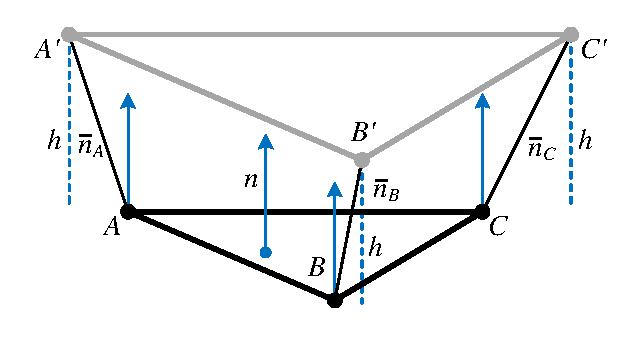
\includegraphics[width=0.65\textwidth]{./fig/3dr_pyramid_partial.pdf}
\singlespacing
\captionstyle{center}\caption{Заметаемый объем при движении узлов треугольника.}
\label{fig:text_1_geo_prim_pyramid_partial}
\end{figure}

Вычисляя положения точек $A'$, $B'$, $C'$ таким же образом, как это было сделано для трапеции в двумерном случае в разделе~\ref{sec:text_1_geo_prim_volume}, можно получить выражение для объема фигуры $ABCA'B'C'$.
\begin{equation}\label{eqn:text_1_geo_prim_abca1b1c1}
	\begin{aligned}
		& \overline{A}' = \overline{A} + h \overline{u}_A, \ \overline{u}_A = \frac{\overline{n}_A}{(\overline{n}_A, \overline{n})} \\
		& \overline{B}' = \overline{B} + h \overline{u}_B, \ \overline{u}_B = \frac{\overline{n}_B}{(\overline{n}_B, \overline{n})} \\
		& \overline{C}' = \overline{C} + h \overline{u}_C, \ \overline{u}_C = \frac{\overline{n}_C}{(\overline{n}_C, \overline{n})} \\
		& S_{ABC} = \frac{1}{2} \Vert (\overline{B} - \overline{A}) \times (\overline{C} - \overline{A}) \Vert \\
		& S_{A'B'C'} = \frac{1}{2} \Vert (\overline{B'} - \overline{A'}) \times (\overline{C'} - \overline{A'}) \Vert \\
		& V_{ABCA'B'C'}(h) = \frac{1}{3} \left( S_{ABC} + \sqrt{S_{ABC} S_{A'B'C'}} + S_{A'B'C'} \right) h
	\end{aligned}
\end{equation}

Полученное в \eqref{eqn:text_1_geo_prim_abca1b1c1} выражение $V_{ABCA'B'C'}(h)$ является кубической функцией от $h$, поэтому $h$ может быть выражено через $V_{ABCA'B'C'}$ путем решения кубического уравнения.

\subsubsection{Метод пирамид}

Второй метод перестроения поверхностной расчетной сетки будем называть методом пирамид, он проиллюстрирован на рис.~\ref{fig:text_1_remesh3_rect} справа (в двумерной постановке аналогом этого метод является метод трапеций).
Входными данными также является объем накопленного льда в каждой ячейке сетки ($V_F$).
Однако в отличие от метода призм объем накопленного в ячейке льда представляется не призмой, а призматоидом, основанием которого является ячейка, а боковые ребра направлены вдоль нормалей узлов (мы будем условно называть эту фигуру усеченной пирамидой, чтобы не путать с методом призм, хотя в общем случае она усеченной пирамидой не является -- прямые, содержащие нормали трех инцидентных этой ячейке узлов, не обязаны пересекаться в одной точке).
Высота этой фигуры ищется из соотношений \eqref{eqn:text_1_geo_prim_abca1b1c1} с помощью решения кубического уравнения (решением является наименьший неотрицательный корень этого кубического уравнения).
Тогда как узлы ячейки являются точками первого основания построенной пирамиды, точки второго основания представляют собой новые положения узлов, вычисленные относительно рассматриваемой ячейки.
Таким образом, у каждого узла сетки вычисляется несколько новых положений (каждое из которых вычислено относительно своей инцидентной ячейки).
Для двумерного случая получается ровно два таких новых положения (так как в двумерном случае каждый узел имеет ровно две инцидентные ячейки), для трехмерного случае таких точек более двух ($|\mathscr{F}(N)|$ штук).
Для выбора единственного нового положения узла сетки берется среднее значение из всех положений, вычисленных относительно инцидентных ячеек.

\subsubsection{Многослойное перестроение поверхностной сетки}

Вне зависимости от используемого метода перестроения значительно повысить точность перестроения можно с помощью многослойного подхода \cite{BourgaultCote2017}.

\begin{figure}[ht]
\centering
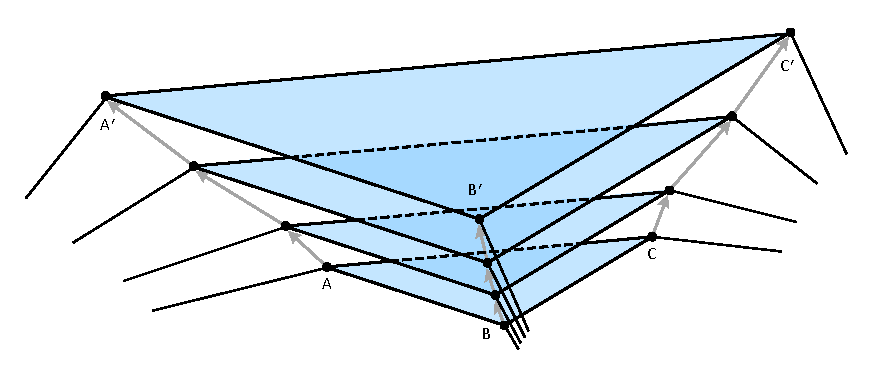
\includegraphics[width=0.6\textwidth]{fig/3dr_classical_methods_multilayer_3d.pdf}
\singlespacing
\captionstyle{center}\caption{Многослойное перестроение сетки.}
\label{fig:text_1_remesh3_multi}
\end{figure}

В этом случае вместо однократного перестроения сетки по объему накопленного льда в каждой ячейке ($V_F$), выбирается фиксированное количество шагов перестроения $k$, а дальше процедура выполняется $k$ раз подряд, но с использованием объема накопленного в ячейке льда $\frac{V_F}{k}$.
Точность повышается из-за того, что после каждого шага перестроения нормали в узлах сетки меняют свое направление, и общий объем наращиваемого льда становится более криволинейным, лучше учитывает геометрию сетки и, как следствие, точнее соответствует исходному значению $V_F$ (см. рис.~\ref{fig:text_1_remesh3_multi}).

Для многослойного метода перестроения может быть применена коррекция с учетом фактически заметенного объема движущейся ячейкой при перестроении поверхности.
Пусть по-прежнему используется многослойный подход с $k$ шагами перестроения (с номерами шагов $i \in [0, k - 1]$).
Кроме объема накопленного льда в ячейке $V_F$ будем также сохранять фактически построенный объем на предыдущий шагах перестроения в переменной $V'_F$, которая перед перестроением равна нулю.
Тогда на $i$-ом шаге перестроения используется целевой объем $\frac{V_F - V'_F}{k - i}$, а переменная $V'_F$ увеличивается на объем фактически построенного льда на этом шаге ($V_{ABCA'B'C}$).
При использовании коррекции в многослойном методе перестроения общая точность совпадает с точностью перестроения на последнем шаге с номером $k - 1$.
Заметим, что при использовании коррекции перестроение может закончить работу досрочно при условии $V_F \le V'_F$ после некоторого шага перестроения.

\subsubsection{Перестроение поверхности со сглаживаниями}\label{sec:tong_method}

В работах \cite{Thompson2013Remesh,Tong2017Remesh} приведено описание итерационного алгоритма эволюции поверхностной сетки, в котором на каждой итерации используются различные виды сглаживания.
Будем называть его методом перестроения Tong.
В нем используется ряд улучшений по сравнению с классическими методами.

Многослойный подход, реализованный в этом методе, не использует константное количество шагов -- величина наращиваемого объема на каждом шаге алгоритма рассчитывается исходя из максимально допустимой доли обледенения, после превышения которого возможно развитие численной нестабильности в эволюции поверхности.
То есть при перестроении расчетной сетки на текущем шаге вместо полного объема накопленного льда в ячейках $V_F$ используется только часть накопленного льда $\alpha V_F$ ($0 < \alpha \le 1$), не приводящая к аварийному завершению перестроения (после этого перестроение продолжается с оставшимся объемом льда).
Наиболее очевидный случай численной нестабильности возникает, когда проекции нормалей узлов на общую инцидентную ячейку пересекаются, в этом случае слишком большой шаг по времени приведет к самопересечению сетки.
Чтобы идентифицировать ячейки, которые будут демонстрировать подобное поведение на текущем временном шаге, предполагается, что объем, образованный путем вытягивания треугольной ячейки с использованием параллельной плоскости смещения, образует призматоид, объем которого определяется кубической функцией высоты $H$ нарастания льда в ячейке
\begin{equation}\label{text_1_remesh_3d_tong1}
	V(H)=aH+bH^2+cH^3.
\end{equation}
где константы $a$, $b$, $c$ определяются позициями узлов грани, их нормалей и нормалью грани (вычисление этих коэффициентов приведено в \eqref{eqn:text_1_geo_prim_abca1b1c1}.

Рассмотрим корни квадратного уравнения, которое получается в результате дифференцирования уравнения \eqref{text_1_remesh_3d_tong1}.
Если корни являются положительными вещественными значениями, то наименьший положительный корень определяет высоту, на которой достигается максимальный объем для рассматриваемой ячейки $F$, не приводящий к возникновению численной нестабильности, который обозначается как $V_F^{max}$, иначе функция $V(H)$ монотонно возрастает и ограничение на шаг по времени в ячейке $F$ не требуется.
Исходя из этого, можно вычислить максимальную долю обледенения, которая требуется для обеспечения устойчивого перестроения.
В дополнение к этому пределу размера шага вводится предел стабильности $\alpha_{jiao}$, который основан на том, как изменяются направления нормалей по мере эволюции поверхности \cite{Jiao2007Offsetting}.
Тогда, допустимая доля для $i$-й ячейки определяется как
\begin{equation}
\alpha_F =
	\begin{cases}
		\min \left( s \frac{V_F^{max}}{V_F}, \alpha_{jiao}, 1 \right), \ V_F^{max} \ne \infty, \\
		\alpha_{jiao}, \ V_F^{max} = \infty
	\end{cases}
\end{equation}
где $s$ ($0 < s < 1$) -- эмпирически определяемый коэффициент, $V_F$ -- целевой объем приращения льда для ячейки $F$.
Тогда объем, наращиваемый для текущего шага, равен $\alpha V_F$, где $\alpha$ представляет собой глобальное минимальное значение для всех ячеек.

Другой важной особенностью алгоритма является введение первичного и нулевого пространств \cite{Jiao2006Smooth}.
Если эволюционное движение узлов сетки происходит в первичном пространстве, то их перемещение в нулевом пространстве будет сохранять заметаемый объем, благодаря чему мы можем  проводить сглаживание поверхности сетки с сохранением объема.

В алгоритме используется несколько видов сглаживаний.
Первое сглаживание -- сглаживание нормалей в узлах и ячейках сетки.
Перемещение узлов при наращивании льда происходит только по их нормалям.
По мере эволюции, на поверхности может усиливаться шум -- если его не контролировать, может возникнуть ситуация, когда двугранный угол между гранями станет слишком малым и ограничит максимальную долю обледенения.
Для уменьшения поверхностного шума, перед наращиванием льда применяется локальное сглаживание, регулирующее направление смещения узлов в проблемных областях, чтобы оно более точно совпадало с направлениями его соседей.
Этот метод может улучшить гладкость поверхности в некоторых ситуациях.

\begin{figure}[ht]
\centering
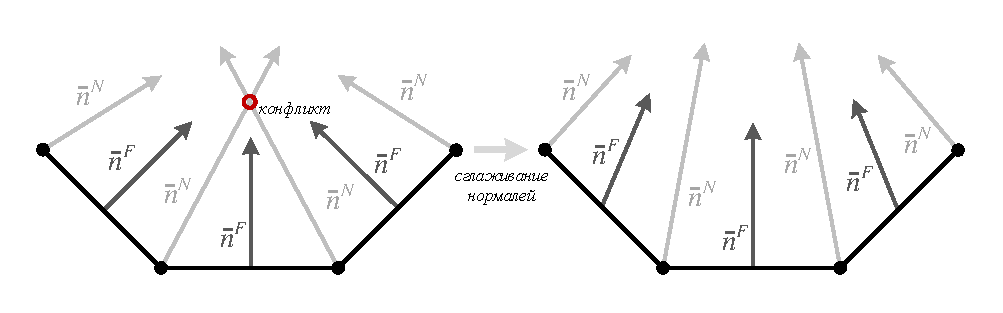
\includegraphics[width=0.8\textwidth]{fig/3dr_normals_smooth.pdf}
\singlespacing
\captionstyle{center}\caption{Сглаживание нормалей.}
\label{fig:text_1_remesh3_normals_smooth}
\end{figure}

Основная цель сглаживания нормалей -- вытолкнуть точки из вогнутых областей, где нормали могут локально сходиться.
Сглаживание нормалей достигается с помощью серий взвешенных средних, которые предназначены для придания веса нормалям, генерируемым проблемными областями.
То есть применяется ряд итераций, во время которых направления смещения ячеек определяются через направления смешения узлов и наоборот.
На рис.~\ref{fig:text_1_remesh3_normals_smooth} проиллюстировано, как сглаживание нормалей помогает предотвратить возникновение конфликтов (в рассматриваемом случае это сворачивание ячейки) и потенциально увеличивает величину $\alpha$.

Второе сглаживание -- сглаживание высот.
После вычисления доли временного шага и объема, наращиваемого для текущего шага льда, для эволюции поверхности необходимо определить поле высот, которое будет соответствовать этому объему, чтобы по нему определить смещения узлов сетки.
Решение уравнения $V(H_F) = \alpha V_F$ обеспечивает поле начальных высот, которое используется для движения поверхности.
Цель дополнительного шага сглаживания высоты состоит в том, чтобы отфильтровать высокочастотный шум в поле высот за счет уменьшения разницы высот между соседними ячейками.
Как правило, высоты двух треугольных ячеек, имеющих общее ребро, не будут равными.
На этом шаге используется сглаживание высот с сохранением объема путем его перераспределения между соседними ячейками.

\begin{figure}[h]
\centering
\begin{tabular}{ll}
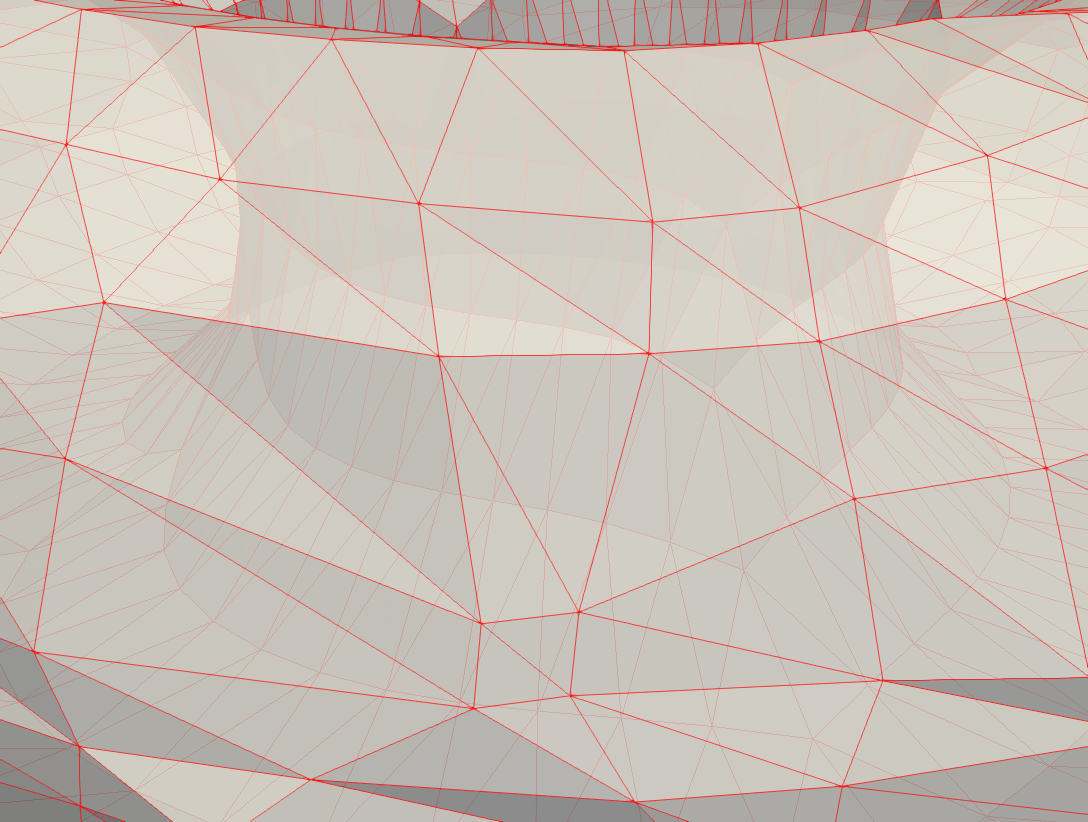
\includegraphics[width=0.45\textwidth]{fig/3dr_smooth_before.png}
&
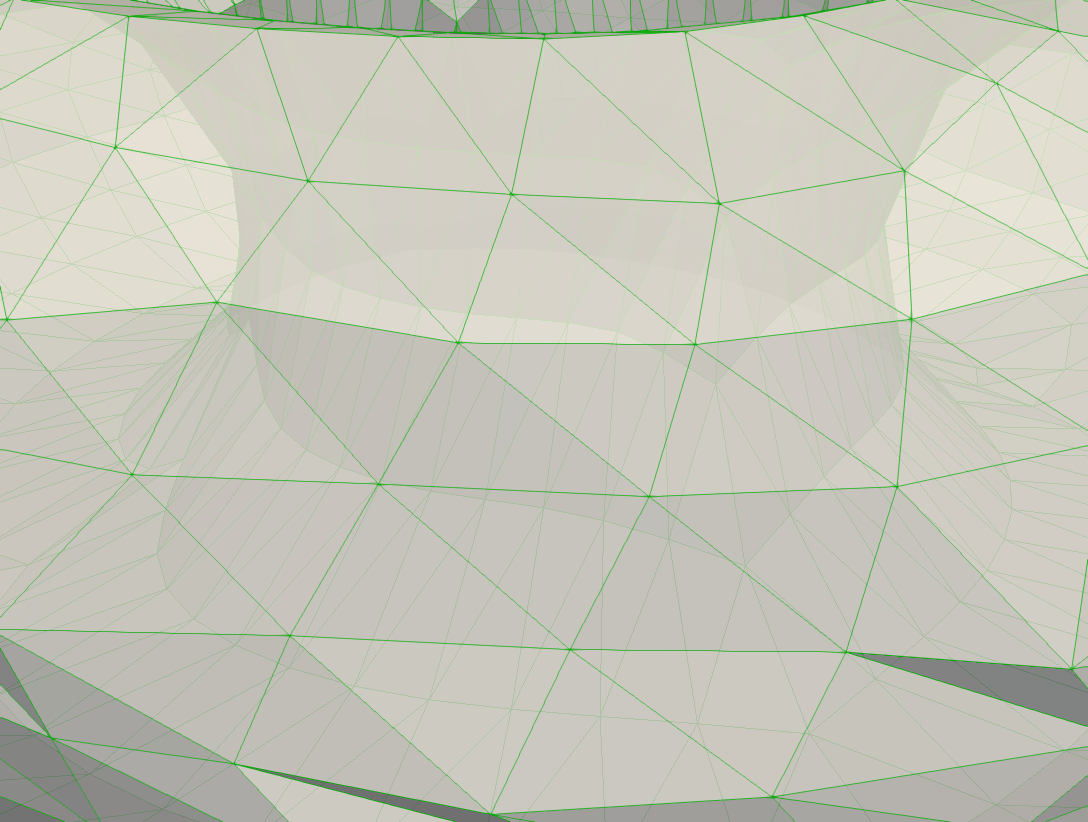
\includegraphics[width=0.45\textwidth]{fig/3dr_smooth_after.png}
\end{tabular}
\singlespacing
\captionstyle{center}\caption{Сглаживание в нулевом пространстве. Вид сетки до сглаживания (слева) и после (справа).}
\label{fig:text_1_remesh3_tong_smooth}
\end{figure}

Последним типом сглаживания является сглаживание в нулевом пространстве.
Эволюция поверхности будет стремиться упаковать узлы в вогнутые области, где сходятся нормали к поверхности, тогда как расширение сетки происходит в выпуклых областях, где нормали к поверхности расходятся.
Если узлы не будут перераспределяться, может стать невозможным продолжать стабильное перестроение сетки (слишком сильное сгущение сетки в вогнутых областям может приводить к конфликтам, а расширение сетки приводит к огрублению сетки).
Для улучшения качества поверхностной сетки узлы перераспределяются на поверхности с помощью сглаживания в нулевом пространстве.
Этот метод способен перераспределять точки, сохраняя при этом целостность базовой геометрии.
Нулевое пространство определяется касательной плоскостью (для гладких областей), касательной линией (для складок поверхностной сетки) или пустым пространством (для углов), движущиеся в нем узлы остаются на поверхности, так что объем и форма поверхности могут быть сохранены (\ref{fig:text_1_remesh3_tong_smooth}).

Отметим, что алгоритм сглаживания может быть распространен на незамкнутые сетки путем закрепления граничных узлов \cite{Shumilin2021Smooth}.

Наиболее слабым местом метода Tong является выбор доли используемого объема $\alpha$ при перестроении.
При возникновении дефектов расчетной сетки (острые пики и впадины) параметр $\alpha$ оказывается близким к нулю даже при использовании сглаживаний нормалей и высот, и время перестроения может неограниченно возрасти.

%---------------------------------------------------------------------------------------------------

\subsection{Метод окрестностей в трехмерном случае}

В этом разделе предлагается метод перестроения поверхностной расчетной сетки, в котором узлы в процессе перестроения смещаются на границу окрестности одной из инцидентных ячеек.
Этот метод перестроения -- метод окрестностей -- является расширением рассмотренного метода окрестностей из раздела~\ref{sec:2dr_okrestnost_method} на трехмерный случай.

Рассмотрим геометрическую задачу определения новых положений узлов расчетной сетки, если для каждого узла $N$ известна скорость увеличения толщины ледяного покрова $v_N$ \cite{Rybakov2023GeoRemesh}.
Будем считать, что нарастание льда в любой точке роста льда выполняется одновременно во всех направлениях аналогично принципу Гюйгенса-Френеля распространения волн.
Таким образом, ОРЛ\label{abbr:orl-2} произвольной точки $P$ через промежуток времени $\Delta t$ будет иметь форму шара $Ball(P, v_P \Delta t)$.
Далее будем считать, что мы выполняем расчет новых положений узлов через некоторый фиксированный момент времени $\Delta t$, то есть для каждого узла $N$ известен радиус ОРЛ $R_N = v_N \Delta t$.
Так как при выполнении численных расчетов обледеневающая поверхность представлена неструктурированной поверхностной расчетной сеткой, ячейки которой имеют форму треугольников, а радиусы ОРЛ заданы только в узлах сетки, необходимо определить радиусы ОРЛ для каждой точки внутри ячейки.

\subsubsection{Поставка задачи для отдельной ячейки}

Рассмотрим некоторую ячейку расчетной сетки, представляющую собой треугольник $Tri(A, B, C)$.
Определим для каждой точки $P(\beta,\gamma)$ внутри треугольника радиус ОРЛ как
\begin{equation}
	R(P(\beta,\gamma)) = R(\beta,\gamma) = R(A) + \beta(R(B) - R(A)) + \gamma(R(C) - R(A))
\end{equation}
и ОРЛ точки $P(\beta,\gamma)$ представляет собой шар $Ball(P(\beta,\gamma), R(\beta,\gamma))$.
ОРЛ всей ячейки расчетной сетки является окрестность этой ячейки $O_R(ABC)$ (см. рис.~\ref{fig:text_1_remesh_common_envelope_1}).

\begin{figure}[ht]
\centering
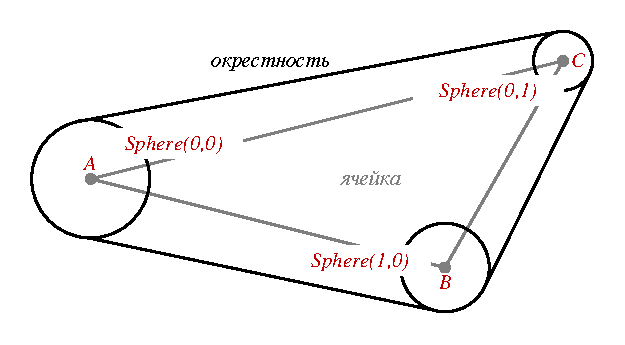
\includegraphics[width=0.6\textwidth]{fig/3dr_triangle.pdf}
\singlespacing
\captionstyle{center}\caption{Окрестность ячейки расчетной сетки.}
\label{fig:text_1_remesh_common_envelope_1}
\end{figure}

При изменении положения узлов расчетной ячейки (точки $A$, $B$, $C$) будем исходить из предположения, что новые положения узлов (точки $A'$, $B'$, $C'$) будут находиться на границе окрестности ячейки $O_R(ABC)$ (пока в расчете не учитываем влияние соседних расчетных ячеек).
Без ограничения общности можно рассмотреть только одну вершину расчетной ячейки (точка $A$).
Пусть траектория движения точки $A$ описывается уравнением полупрямой $\overline{P}(\alpha) = \overline{A} + \alpha \overline{D}$ при $\alpha \ge 0$ ($\overline{D}$ -- вектор направления движения точки, при этом можно считать $|\overline{D}| = 1$).

Для поиска точек пересечения траектории движения точки $\overline{P}(\alpha) = \overline{A} + \alpha \overline{D}$ с 
произвольной сферой $Sphere(\beta,\gamma)$ необходимо подставить координаты точки $\overline{P}(\alpha)$ в уравнение сферы $|\overline{P} - \overline{C}(\beta,\gamma)| = R(\beta,\gamma)$, где $\overline{C}(\beta,\gamma)$ -- ее центр.
В результате получим уравнение
\begin{equation}\label{eqn:text_1_remesh_common_envelope_eq}
	|(\overline{A} + \alpha \overline{D}) - \overline{C}(\beta, \gamma)| = R(\beta, \gamma)
\end{equation}

Уравнение \eqref{eqn:text_1_remesh_common_envelope_eq} решается относительно неизвестной $\alpha$ при фиксированных параметрах $\beta$, $\gamma$.
Это уравнение является квадратным, оно имеет не более двух корней, которые будем рассматривать как функцию с двумя параметрами $\alpha_{1,2} = \alpha_{1,2}(\beta,\gamma)$.
Для определения нового положения точки $A$ необходимо найти максимальное значение вещественного корня такого уравнения для всех допустимых значений параметров $\beta$ и $\gamma$:
\begin{equation}
\alpha = \max_{\substack{\beta \ge 0, \ \gamma \ge 0 \\ \beta + \gamma \le 1}}{\alpha_{1,2}(\beta, \gamma)}
\end{equation}

При этом точка пересечения траектории движения точки $A$ с границей окрестности ячейки $O_R(ABC)$ может находиться на разных участках этой границы, что продемонстрировано на рис.~\ref{fig:text_1_remesh_common_envelope_2} и связано с условиями, которым удовлетворяют параметры $\beta$, $\gamma$ (а, б, в -- пересечение со сферой с центром в вершинах треугольника; г, д, е -- пересечение со сферой с центром на ребрах треугольника, g -- пересечение со сферой с центром внутри треугольника).

\begin{figure}[ht]
\centering
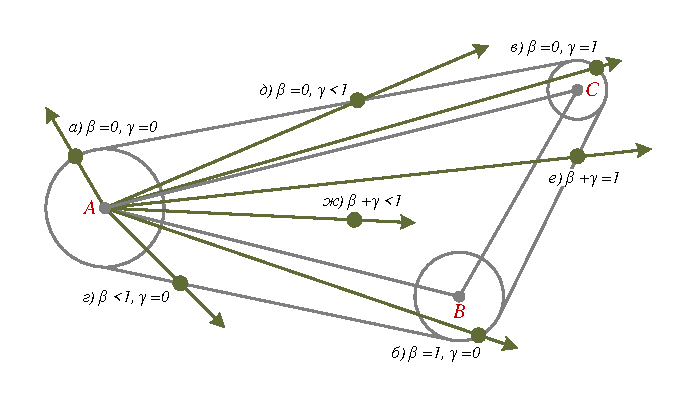
\includegraphics[width=0.6\textwidth]{fig/3dr_triangle2.pdf}
\singlespacing
\captionstyle{center}\caption{Различные варианты пересечения траектории смещения узла и окрестности ячейки.}
\label{fig:text_1_remesh_common_envelope_2}
\end{figure}

Введем следующие обозначения $R_A = R(A)$, $R_{AB} = R(B) - R(A)$, $R_{AC} = R(C) - R(A)$, тогда \eqref{eqn:text_1_remesh_common_envelope_eq} можно записать в виде
\begin{equation}
	|\alpha \overline{D} - (\beta \overline{AB} + \gamma \overline{AC})|^2 = (R_A + \beta R_{AB} + \gamma R_{AC})^2,
\end{equation}
или явно как квадратное уравнение относительно переменной $\alpha$:
\begin{multline}
	|\overline{D}|^2 \alpha^2 - 2(\beta (\overline{D}, \overline{AB}) + \gamma (\overline{D}, \overline{AC})) \alpha + \\
	|\beta \overline{AB} + \gamma \overline{AC}|^2 - (R_A + \beta R_{AB} + \gamma R_{AC})^2 = 0
\end{multline}

Наибольший корень этого квадратного уравнения вычисляется следующим образом (с учетом условия $|\overline{D}| = 1$):
\begin{multline}
	\alpha(\beta, \gamma) = \beta (\overline{D}, \overline{AB}) + \gamma (\overline{D}, \overline{AC}) + \\
	\sqrt{(\beta (\overline{D}, \overline{AB}) + \gamma (\overline{D}, \overline{AC}))^2 - |\beta \overline{AB} + \gamma \overline{AC}|^2 + (R_A + \beta R_{AB} + \gamma R_{AC})^2},
\end{multline}
или
\begin{equation}\label{eqn:3dr_okrestnost_full_eqn}
	\begin{aligned}
		& \alpha(\beta, \gamma) = k_{\beta} \beta + k_{\gamma} \gamma + \sqrt{T} \\
		& T = q_{\beta^2} \beta^2 + q_{\gamma^2} \gamma^2 + q_{\beta \gamma} \beta \gamma + q_{\beta} \beta + q_{\gamma} \gamma + q \\
		& k_{\beta} = (\overline{D}, \overline{AB}), \ k_{\gamma} = (\overline{D}, \overline{AC}) \\
		& q_{\beta^2} = (\overline{D}, \overline{AB})^2 - |\overline{AB}|^2 + R_{AB}^2, \ q_{\gamma^2} = (\overline{D}, \overline{AC})^2 - |\overline{AC}|^2 + R_{AC}^2 \\
		& q_{\beta \gamma} = 2 \left( (\overline{D}, \overline{AB}) (\overline{D}, \overline{AC}) - (\overline{AB}, \overline{AC}) + R_{AB}R_{AC} \right) \\
		& q_{\beta} = 2 R_A R_{AB}, \ q_{\gamma} = 2 R_A R_{AC}, \ q = R_A^2
	\end{aligned}
\end{equation}

\subsubsection{Задача поиска точек пересечения прямой с окрестностью отрезка}\label{sec:text_1_geo_prim_line_eps_intersect}

Для поиска решений уравнения~\eqref{eqn:3dr_okrestnost_full_eqn} для всех вариантов допустимых параметров $\beta$ и $\gamma$, представленных на рис.~\ref{fig:text_1_remesh_common_envelope_2}, рассмотрим задачу поиска точек пересечения прямой с окрестностью отрезка \cite{Rybakov2017Flight}.

Пусть в пространстве задан отрезок $Segm(A, B)$.
Рассмотрим его окрестность $O_R(Segm(A, B))$, где функция $R$ задана на точках этого отрезка $\overline{C}(\alpha) = \overline{A} + \alpha \overline{AB}, \ 0 \le \alpha \le 1$ следующим образом:
\begin{equation}
	\left\{
		\begin{aligned}
			& R(A) = R_A \\
			& R(B) = R_B \\
			& R(C(\alpha)) = R(\alpha) = R_A + \alpha (R_B - R_A) = R_A + \alpha \Delta R
		\end{aligned}
	\right.
\end{equation}

Также пусть в пространстве задана прямая.
Без ограничения общности можно считать, что эта прямая проходит через начало координат, пусть она имеет вид $Line(\overline{0}, \overline{V}) = \{ \overline{P}(\tau) = \tau \overline{V}: \tau \in \mathbb{R} \}$.

Требуется найти точки пересечения прямой $Line(\overline{0}, \overline{V})$ и окрестности отрезка $O_R(Segm(A, B))$.

Точки пересечения прямой $Line(\overline{0}, \overline{V})$ и сферы $Sphere(C, R)$ находятся из решения системы уравнений
\begin{equation}\label{eqn:text_1_geo_prim_tv_pcr}
	\left\{
		\begin{aligned}
			& \overline{P} = \tau \overline{V} \\
			& |\overline{P} - \overline{C}| = R^2
		\end{aligned}
	\right.
\end{equation}

Система уравнений \eqref{eqn:text_1_geo_prim_tv_pcr} преобразуется в квадратное уравнение относительно $\tau$, дискриминант которого равен $4\left((\overline{C}, \overline{V})^2 - |\overline{V}|^2 \left(|\overline{C}|^2 - R^2\right)\right)$.
Общие точки прямой и сферы существуют если этот дискриминант неотрицателен.

Аналогично, точки пересечения прямой $Line(\overline{0}, \overline{V})$ и сферы с центром в точке $C(\alpha)$ и радиусом $R(\alpha)$ существуют, если выполняется условие
\begin{equation}
	(\overline{C}(\alpha), \overline{V})^2 - |\overline{V}|^2 \left(|\overline{C}(\alpha)|^2 - R(\alpha)^2\right) \ge 0.
\end{equation}

Подставив конкретные выражения для центра и радиуса сферы, получим квадратное неравенство относительно параметра $\alpha$:
\begin{equation}\label{eqn:text_1_geo_prim_ineq_k2k1k0}
	k_2 \alpha^2 + 2 k_1 \alpha + k_0 \ge 0,
\end{equation}
где
\begin{equation}\label{eqn:text_1_geo_prim_k2k1k0}
	\begin{aligned}
		& k_2 = (\Delta \overline{C}, \overline{V})^2 + |\overline{V}|^2 \left( \Delta R^2 - |\Delta \overline{C}|^2 \right) \\
		& k_1 = (\overline{C}_A, \overline{V})(\Delta \overline{C}, \overline{V}) + |\overline{V}|^2 \left(R_A \Delta R - (\overline{C}_A, \Delta \overline{C}) \right) \\
		& k_0 = (\overline{C}_A, \overline{V})^2 + |\overline{V}|^2 \left( R_A^2 - |\overline{C}_A|^2 \right)
	\end{aligned}
\end{equation}

В системе \eqref{eqn:text_1_geo_prim_k2k1k0} для удобства введены обозначения $C_A = A$, $\Delta \overline{C} = \overline{AB}$.

Неравентво \eqref{eqn:text_1_geo_prim_ineq_k2k1k0} может быть решено относительно $\alpha$, так как все коэффициенты из \eqref{eqn:text_1_geo_prim_k2k1k0} могут быть вычислены непосредственно.
Нас интересует решение неравенства \eqref{eqn:text_1_geo_prim_ineq_k2k1k0} только на отрезке $[0,1]$, оно представляет собой либо пустое множество, либо отрезок.
Если на отрезке $[0,1]$ неравенство \eqref{eqn:text_1_geo_prim_ineq_k2k1k0} не имеет решения, то прямая $Line(\overline{0}, \overline{V})$ не пересекает $O_R(Segm(A, B))$.
Допустим на отрезке $[0,1]$ неравенство \eqref{eqn:text_1_geo_prim_ineq_k2k1k0} имеет решение $[\alpha_0, \alpha_1] \subseteq [0, 1]$.
 
Для произвольного $\alpha \in [\alpha_0, \alpha_1]$ корни уравнения
\begin{equation}
	|\overline{V}|^2 \tau^2 - 2(\overline{C}(\alpha), \overline{V}) \tau + \left( |\overline{C}(\alpha)| - R(\alpha)^2 \right) = 0
\end{equation}
существуют и выражаются следующим образом:
\begin{equation}
	\tau_{2,1}(\alpha) = \frac{(\overline{C}(\alpha), \overline{V}) \pm \sqrt{k_2 \alpha^2 + 2 k_1 \alpha + k_0}}{|\overline{V}|^2}.
\end{equation}

Искомые точки пересечения прямой $Line(\overline{0}, \overline{V})$ с границей окрестности отрезка $O_R(Segm(A, B))$ соответствуют минимальному и максимальному значениям параметра $\tau_{1,2}(\alpha)$, достигаемым на отрезке $[\alpha_0, \alpha_1]$.
Минимальное и максимальное значение $\tau_{1,2}(\alpha)$ могут достигаться либо на концах отрезка, либо в точках локального экстремума.
Для точки локального экстремума должно быть выполнено условие $\tau_{1,2}'(\alpha) = 0$ или в явном виде
\begin{equation}
	(\Delta \overline{C}, \overline{V}) \pm \frac{k_2 \alpha + k_1}{ \sqrt{k_2 \alpha^2 + 2 k_1 \alpha + k_0} } = 0.
\end{equation}

Введя обозначение $q = (\Delta \overline{C}, \overline{V})^2$, получим квадратное уравнение относительно $\alpha$:
\begin{equation}
	k_2 (k_2 - q) \alpha^2 + 2 k_1 (k_2 - q) \alpha + (k_1^2 - q k_0) = 0,
\end{equation}
решая которое, получим потенциальные точки локальных экстремумов, которые обозначим $\tilde{\alpha}_1$, $\tilde{\alpha}_2$.

Точки $\tilde{\alpha}_1$, $\tilde{\alpha}_2$ нужно учитывать только если они попадают в отрезок $[\alpha_0, \alpha_1]$.
В общем случае значения $\tau_{1,2}$ находятся по четырем значениям $\alpha$
\begin{equation}
	\left\{
		\begin{aligned}
			\tau_1 = \min(\tau_{1}(\alpha_0), \tau_{1}(\alpha_1), \tau_{1}(\tilde{\alpha}_1), \tau_{1}(\tilde{\alpha}_2)) \\
			\tau_2 = \max(\tau_{2}(\alpha_0), \tau_{2}(\alpha_1), \tau_{2}(\tilde{\alpha}_1), \tau_{2}(\tilde{\alpha}_2))
		\end{aligned}
	\right.
\end{equation}

Множеством общих точек $Line(\overline{0}, \overline{V})$ и $O_R(Segm(A, B))$ является $\{ \overline{P}(\tau) = \tau \overline{V}: \tau_1 \le \tau \le \tau_2 \}$ (см. рис.~\ref{fig:text_1_geo_prim_spheres_nest_intersection}).

\begin{figure}[ht]
\centering
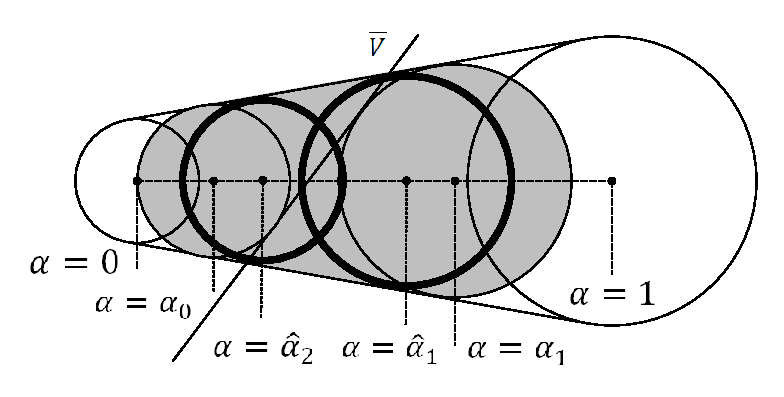
\includegraphics[width=0.6\textwidth]{fig/3dr_spheres_nest_intersection.pdf}
\singlespacing
\captionstyle{center}\caption{Пересечение прямой с окрестностью отрезка.}
\label{fig:text_1_geo_prim_spheres_nest_intersection}
\end{figure}

\subsubsection{Поиск нового положения узла сетки}

Для поиска нового положения точки $A$ требуется найти максимум выражения $\alpha(\beta,\gamma)$ из \eqref{eqn:3dr_okrestnost_full_eqn} при условии соблюдения ограничений $\beta \ge 0$, $\gamma \ge 0$, $\beta + \gamma \le 1$.
Максимум выражения $\alpha(\beta, \gamma)$ достигается либо при условии нахождения центра сферы внутри треугольника $ABC$ , либо на одной из его сторон.
В случае нахождения центра сферы на стороне $AB$ треугольника $ABC$ выполняется условие $\gamma = 0$, и выражение для величины $\alpha$ имеет вид
\begin{equation}
	\alpha_{\gamma = 0} = k_{\beta} \beta + \sqrt{q_{\beta^2} \beta^2 + q_{\beta} \beta + q}.
\end{equation}

В случае нахождения центра сферы на стороне $AC$ треугольника $ABC$ выполняется условие $\beta = 0$, и выражение для величины $\alpha$ имеет вид
\begin{equation}
	\alpha_{\beta = 0} = k_{\gamma} \gamma + \sqrt{q_{\gamma^2} \gamma^2 + q_{\gamma} \gamma + q}.
\end{equation}

В случае нахождения центра сферы на стороне $BC$ треугольника $ABC$ выполняется условие $\beta + \gamma = 1$, и выражение для величины $\alpha$ имеет вид
\begin{multline}
	\alpha_{\beta + \gamma = 1} = (k_{\gamma} - k_{\beta}) \gamma + k_{\beta} + \\
	\sqrt{(q_{\beta^2} + q_{\gamma^2} + q_{\beta \gamma}) \gamma^2 + (-2 q_{\beta^2} + q_{\beta \gamma} - q_{\beta} + q_{\gamma}) \gamma + (q_{\beta^2} + q_{\beta} + q)}.
\end{multline}

Во всех случаях нахождения центра сферы на одной из сторон треугольника задача нахождения максимального значения $\alpha(\beta, \gamma)$ при заданных ограничениях сводится к задаче поиска максимального значения функции вида $\alpha(x) = k_x x + k + \sqrt{q_{x^2} x^2 + q_x x + q}$ (с учетом этих ограничений), что является аналогом задачи поиска пересечения прямой и окрестностью отрезка, описание которой приведено в разделе \ref{sec:text_1_geo_prim_line_eps_intersect} (точкой максимума является либо точка локального экстремума, либо точка, находящаяся на границе области определения функции).

Отдельно рассмотрим вариант, когда центр искомой сферы находится внутри треугольника.
В этом случае точка пересечения траектории $\overline{P}(\alpha) = \overline{A} + \alpha \overline{D}$ находится на общей касательной плоскости к сферам $Sphere(0,0)$, $Sphere(1,0)$, $Sphere(0,1)$ (плоскость $A'B'C'$, см. рис.~\ref{fig:text_1_remesh_common_envelope_3}).

\begin{figure}[ht]
\centering
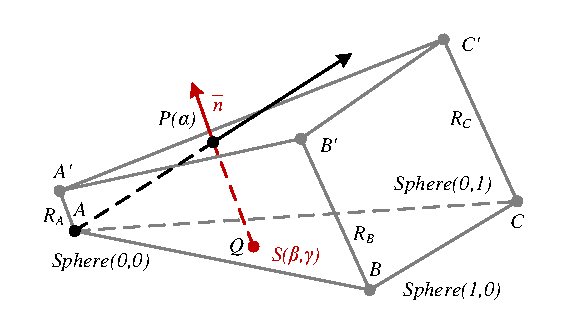
\includegraphics[width=0.7\textwidth]{fig/3dr_case1.pdf}
\singlespacing
\captionstyle{center}\caption{Случай нахождения пересечения траектории движения точки с границе окрестности ячейки, если центр сферы лежит внутри треугольника.}
\label{fig:text_1_remesh_common_envelope_3}
\end{figure}

Центр искомой сферы находится в точке пересечения плоскости $ABC$ и прямой, проходящей через точку $\overline{P}(\alpha)$ и направленной вдоль нормали к плоскости $A'B'C'$ .
Если вектор единичной нормали плоскости $A'B'C'$ обозначить через $\overline{n}$, то взаимосвязь точек плоскостей $ABC$ и $A'B'C'$ можно выразить следующим образом:
\begin{equation}
	\begin{aligned}
		\overline{A}' = \overline{A} + \overline{n}R_A \\
		\overline{B}' = \overline{B} + \overline{n}R_B \\
		\overline{C}' = \overline{C} + \overline{n}R_C
	\end{aligned}
\end{equation}

Для нахождения вектора $\overline{n}$ используем тот факт, что результат векторного произведения $\overline{A'B'} \times \overline{A'C'}$ коллинеарен вектору $\overline{n}$.
Запишем это в явном виде
\begin{equation}
	(\overline{AB} + \overline{n} R_{AB}) \times (\overline{AC} + \overline{n} R_{AC}) = t \overline{n}
\end{equation}

\begin{equation}
	\overline{AB} \times \overline{AC} + R_AB(\overline{n} \times \overline{AC}) - R_{AC}(\overline{n} \times \overline{AB}) = t \overline{n}
\end{equation}

\begin{equation}\label{eqn:text_1_remesh_common_envelope_matr}
	t
	\begin{pmatrix}
		n_x \\
		n_y \\
		n_z
	\end{pmatrix}
	+ R_{AC}
	\begin{pmatrix}
		n_y AB_z - n_z AB_y \\
		n_z AB_x - n_x AB_z \\
		n_x AB_y - n_y AB_x
	\end{pmatrix}
	- R_{AB}
	\begin{pmatrix}
		n_y AC_z - n_z AC_y \\
		n_z AC_x - n_x AC_z \\
		n_x AC_y - n_y AC_x
	\end{pmatrix}
	= \overline{AB} \times \overline{AC}
\end{equation}

Соотношение \eqref{eqn:text_1_remesh_common_envelope_matr} может выполняться как при $t > 0$, так и при $t < 0$, что соответствует существованию двух общих касательных плоскостей к трем сферам.
Перепишем приведенное соотношение в виде системы линейных уравнений относительно составляющих нормали при произвольном значении параметра $t$.
\begin{multline}\label{eqn:text_1_remesh_common_envelope_matr2}
	\begin{pmatrix}
		t                         & R_{AC} AB_z - R_{AB} AC_z & R_{AB} AC_y - R_{AC} AB_y \\
		R_{AB} AC_z - R_{AC} AB_z & t                         & R_{AC} AB_x - R_{AB} AC_x \\
		R_{AC} AB_y - R_{AB} AC_y & R_{AB} AC_x - R_{AC} AB_x & t
	\end{pmatrix}
	\begin{pmatrix}
		n_x \\
		n_y \\
		n_z
	\end{pmatrix} \\
	= \overline{AB} \times \overline{AC}
\end{multline}

Из системы уравнений \eqref{eqn:text_1_remesh_common_envelope_matr2} находятся два возможных направления нормали к общей касательной плоскости для сфер $Sphere(0,0)$, $Sphere(1,0)$, $Sphere(0,1)$.
Для каждого направления нормали находится плоскость $A'B'C'$ и точка $\overline{P}(\alpha) = \overline{A} + \alpha \overline{D}$ на ней (и сам искомый параметр $\alpha$).
Эту точку можно учитывать в общем наборе решений только в том случае, если ей соответствует сфера $Sphere(\beta, \gamma)$, параметры которой удовлетворяют условиям $\beta \ge 0$, $\gamma \ge 0$, $\beta + \gamma \le 1$.
Параметры $\beta$, и $\gamma$ можно определить путем поиска точки пересечения прямой $Line(P(\alpha), \overline{n})$ и плоскости $ABC$.

\begin{figure}[ht]
\centering
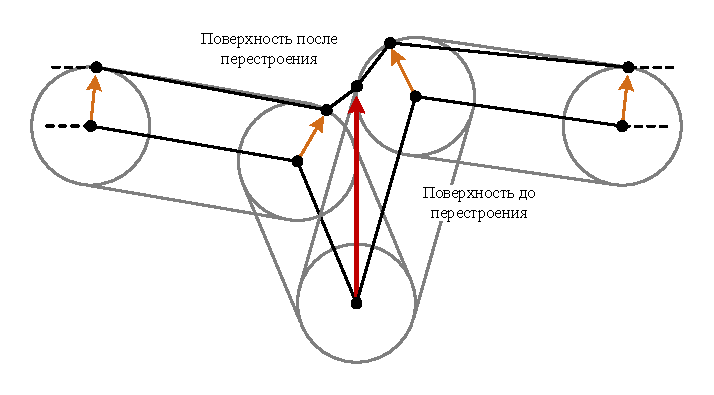
\includegraphics[width=0.7\textwidth]{fig/3dr_out_from_cave.pdf}
\singlespacing
\captionstyle{center}\caption{Выбор наибольшего смещения узла по инцидентным ячейкам.}
\label{fig:text_1_remesh_common_envelope_4}
\end{figure}

Таким образом, найдя решения всех потенциально возможных частных случаев, представленных на рис.~\ref{fig:text_1_remesh_common_envelope_2}, находим множество решений $\alpha$ , из которых для определения актуального нового положения точки $A'$ необходимо выбрать максимальное.
На этом определение смещения узлов расчетной сетки завершено.

Изложенный выше алгоритм касается определения смещения узла с учетом только одной инцидентной ячейки.
При рассмотрении отдельного узла расчетной сетки требуется вычислить смещение этого узла относительно каждой инцидентной ячейки и выбрать среди этих смещений максимальное (см. рис.~\ref{fig:text_1_remesh_common_envelope_4}).

\subsubsection{Анализ метода окрестностей}

Разработанный метод окрестностей перестроения поверхностной расчетной сетки, равно как и его двумерный аналог, обладает способностью сглаживать дефекты сетки -- острые пики и впадины.
Для проверки сглаживания впадин выполнялась проверка метода на тестовых трехмерных моделях, в частности на модели Stanford Bunny \cite{StanfordModels}.

\begin{figure}[ht]
\centering
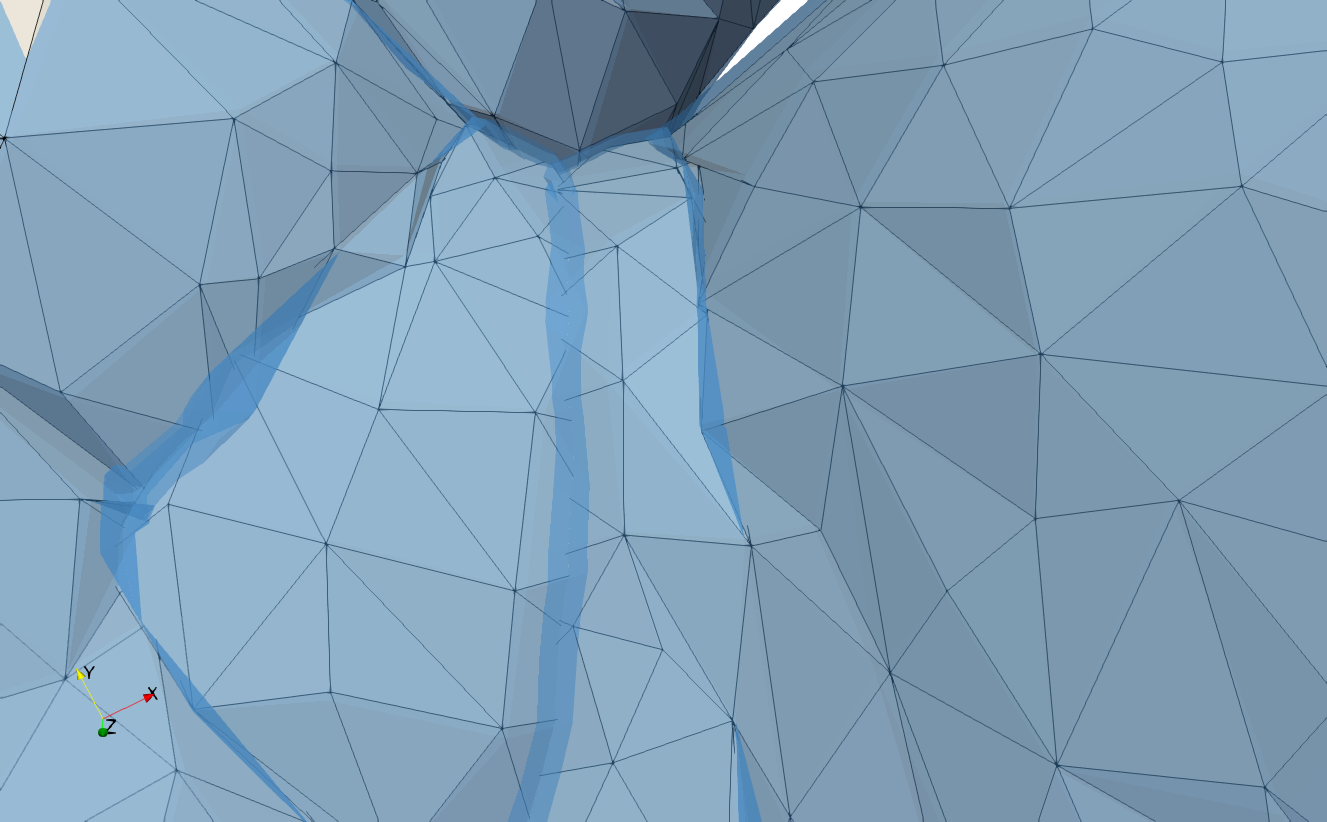
\includegraphics[width=0.45\textwidth]{fig/3dr_bunny_cave.png}
\singlespacing
\captionstyle{center}\caption{Результат работы алгоритма перестроения сетки на тестовой сетке Stanford Bunny.}
\label{fig:text_1_remesh3_common_envelope_bunny}
\end{figure}

На рис.~\ref{fig:text_1_remesh3_common_envelope_bunny} представлен результат сравнения методов призм и окрестностей с точки зрения способности сглаживания впадин.
Светло-синим цветом на рисунке отображена расчетная сетка, перестроенная с помощью метода призм.
Темно-синим цветом показаны участки расчетной сетки, на которых было выполнено сглаживание впадин при перестроении с помощью метода окрестностей с использованием того же объема накопленного в ячейках сетки льда.

Для демонстрации сглаживания острых пиков проводились сравнительные запуски по перестроению расчетной сетки профиля летательного аппарата с помощью программных комплексов FENSAP-ICE (метод призм, многослойное перестроение) и <<Кристалл>> (метод окрестностей, многослойное перестроение).
Результаты перестроения продемонстрированы на рис.~\ref{fig:text_1_remesh3_with_fensap}.

\begin{figure}[!ht]
\centering
\begin{tabular}{ll}
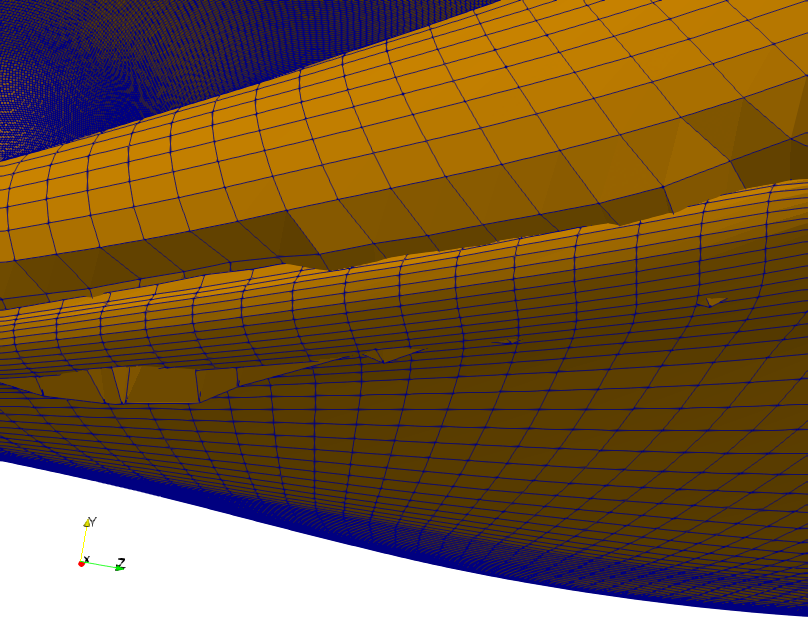
\includegraphics[width=0.43\textwidth]{fig/3dr_fens1.png}
&
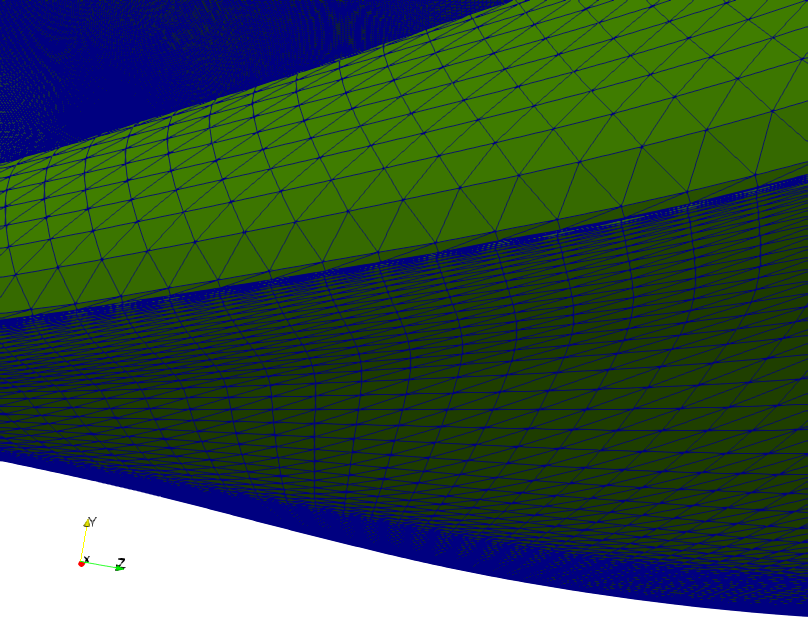
\includegraphics[width=0.43\textwidth]{fig/3dr_crys1.png} \\
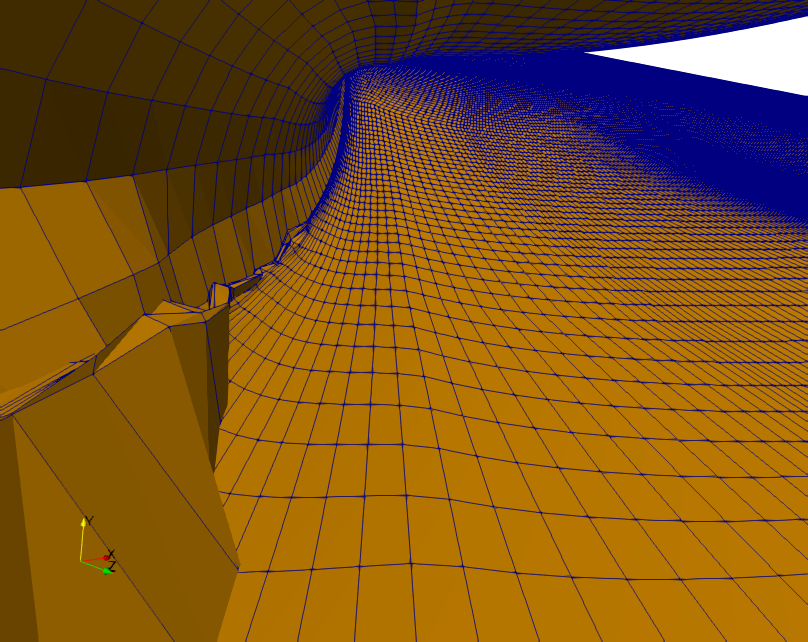
\includegraphics[width=0.43\textwidth]{fig/3dr_fens2.png}
&
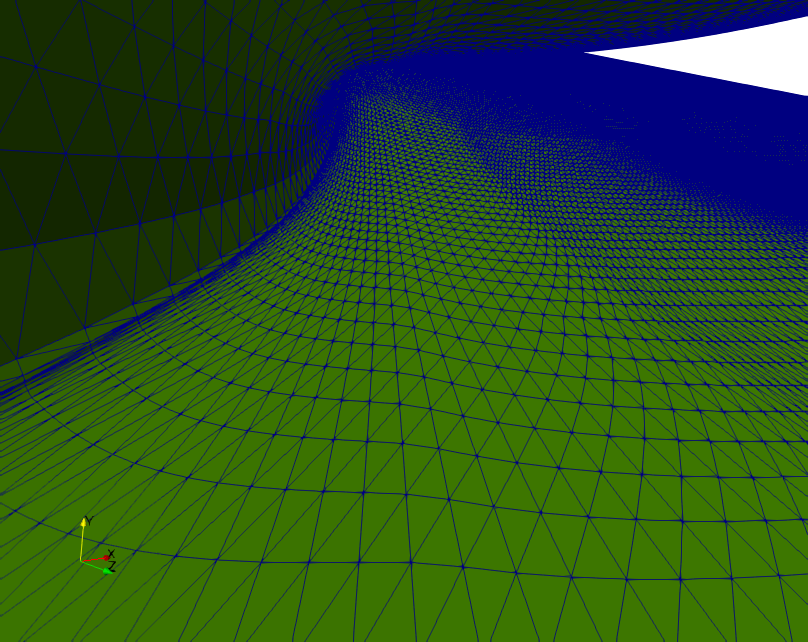
\includegraphics[width=0.43\textwidth]{fig/3dr_crys2.png}
\end{tabular}
\singlespacing
\caption{Эффект сглаживания дефектов при перестроении методом окрестностей (справа) в сравнении с программным комплексом FENSAP-ICE (слева).}
\label{fig:text_1_remesh3_with_fensap}
\end{figure}

На рис.~\ref{fig:text_1_remesh3_with_fensap} слева можно увидеть, что в некоторый момент при перестроении с помощью FENSAP-ICE появились острые пики, которые привели к деформации профиля -- на изображении слева сверху можно видеть, как образовавшиеся острые пики протыкают профиль насквозь.
Подобные дефекты означают невозможность проведения дальнейших расчетов.
На рис.~\ref{fig:text_1_remesh3_with_fensap} справа при перестроении с помощью <<Кристалл>> эффекта возникновения острых пиков не наблюдается, так как используемый метод окрестностей успешно их сглаживает, не приводя к критическим дефектам расчетной сетки.

%---------------------------------------------------------------------------------------------------

\subsection{Выводы из главы}

В главе исследовались методы перестроения поверхностной расчетной сетки в трехмерном случае.
Рассматривалось перестроение сетки при фиксированных направлениях смещения узлов $N$, совпадающих с их нормалями $\overline{n}_{N}^N$.
Рассматривались известные методы перестроения, основанные на приближении целевого объема ячейки $V$ с помощью геометрических примитивов (методы призм и пирамид).
Рассматривались дополнительные аспекты повышения точности и стабильности перестроение расчетной сетки: многослойное перестроение, сглаживание нормалей и высот льда, перераспределение узлов по поверхности.

Предложен новый метод перестрения поверхностной расчетной сетки -- метод окрестностей -- в котором новое положение узла $N'$ определеятся как точка пересечения направления $\overline{n}_{N}^N$ с границей окрестности всех инцидентных узлу ячеек.
Этот метод является обобщением метода окрестностей из первой главы на трехмерный случай.

Продемонстрировано, что метод окрестностей в трехмерной постановке, также как и его двумерный аналог, позволяет сглаживать дефекты расчетной сетки (острые пики и впадины), что обеспечивает стабильность перестроения в процессе моделирования ледообразования.

Стоит отметить, что в реализацию метода окрестностей перестроения поверхностной расчетной сетки были включены некоторые элементы, используемые в других известных методах.
Так было реализовано многослойное перестроение, в помощью которого можно существенно повысить точность.
Также были использованы сглаживание нормалей и высот, с помощью которых можно получить более гладкую расчетную сетку.

По результатам проведенных исследований можно заключить, что предложенный метод окрестностей перестроения поверхностной расчетной сетки является наиболее подходящим для моделирования ледообразования с точки зрения точности перестроения и сглаживания дефектов сетки.

%---------------------------------------------------------------------------------------------------
